\chapter{对超新星遗迹W51C的磁流体模拟及观测分析}
\label{W51C}



\section{研究历史及意义}
\label{W51Cintro}
SNR W51C存在于W51复合区中,除了这个遗迹,这个区域还包括两个电离氢区W51 A/B。
这两个电离氢区尺寸都很大,而且包括很多小一些的电离结构,比如G49.2-0.35。
SNR W51C有很厚的半圆形的单壳层,射电图像尺寸大约为14\am $\times$ 20\am
\citep{Copetti1991,Subrahmanyan1995}。
而且SNR W51C一侧与电离氢区W51B相邻,最近的观测显示在此处有明显的高能特征
\citep{Abdo2009,Aleksic2012},因此我们认为这个遗迹是与分子云相互作用的。
在W51B的东侧,也就是临近W51C的爆发中心,我们探测到了OH的1720MHz脉泽
\citep{Hewitt2008,Brogan2013},这是支持相互作用的另一个证据。
W51A是一个活跃的恒星形成区,但是并没有任何迹象表明与W51C相关,不过和W51B在
一氧化碳(CO)和红外图像上看是互相关联的\citep{Kang2010,Parsons2012,Ginsburg2015}。
两个电离氢区的距离是5 kpc $\sim$ 8 kpc
\citep{Genzel1981,Schneps1981,Xu2009,Sato2010,Tian2013},而SNR W51C的距离是
4.3 kpc \citep{Tian2013} 到 6 kpc \citep{Koo1995}。
这三者的空间关系让我们思考是否它们也有一定物理联系。

之前对这个复合体的观测已经有很多,可是其中主体结构之间的联系依然不清楚。
因此,为了研究遗迹和电离氢区的物理联系,我们决定模拟这个遗迹的磁流体演化,并通过分析
射电偏振数据和OH谱线数据来理解模拟的结果。

\section{数据处理}
\label{W51Cdata}

我们使用的偏振数据来源于Effelsberg 11cm (2.695GHz) 巡天\citep{1999A&A...350..447D}。
这个巡天其实已经展示了W51复合区的偏振图像,可是他们为了图像可以覆盖
更大片区域,使用了较低的分辨率,从而导致一些小结构模糊不清。
原本的分辨率是5\am, 实际展示的是12\am。
在图~\ref{fig:mag}中,我们展示了原始分辨率的偏振图,并旋转偏振方向90$^{\circ}$得到一个
大概的磁场走向。
因为11cm巡天数据存在$0.7\% \pm 0.25\%$的仪器偏振 \citep{1987A&AS...69..451J},我们
不得不先扣除仪器偏振以得到真实偏振强度。
首先,我们在总强度图中扣除了小于一个标准差的值,我们认为这些区域只是不相干的背景,与目标源
无关。
然后我们通过$I^{final}_{pol}=I^{primary}_{pol}-I_{total}*0.007$来计算真实偏振强度,
如果得到负值,我们设其为零,因为这证明这个区域并没有偏振流量。
这里$I^{final}_{pol}$是得到的偏振强度,$I^{primary}_{pol}$是初始观测数据中的偏振强度,
$I_{total}$是总的辐射强度。
最终,我们可以通过$p=I^{final}_{pol}/I_{total}$得到偏振度。
事实上,仪器偏振强度在部分区域可能少于$0.7\%$,所以扣除后的图像中有很多负值。
这个巡天的总流量和偏振灵敏度分辨是20 mK和11 mK,足以帮助我们找到很弱的偏振辐射。

我们使用分辨率较高的THOR DR1数据\citep{Beuther2016},尝试对这个区域的OH辐射进行更详尽的研究。
DR1覆盖了银道坐标中$15^{\circ}<l<67^{\circ}$,$-1^{\circ}<b<1^{\circ}$这大片区域,
包含了1.4GHz连续谱图像,HI、OH (1612/1665/1720 MHz)谱线图和射电复合线谱线图。
其空间分辨率达到了20\as,这是对这一区域的射电巡天项目中最高的分辨率,而其OH谱线的速度分辨率
达到1.5\kms,也是非常高的。
因为这一区域有的OH脉泽谱线非常强,以至于我们无法将其与其他有意义的谱线用同一标度画在一张图
上,所以在脉泽区域我们修改了强脉泽的标度,它们的谱线强度都被人为地除了20。

文中用到的1.4GHz连续谱图像来自于VGPS(VLA Galactic Plane Survey) \citep{Stil2006}.
因为Effelsberg数据的分辨率较低,无法呈现这个区域的细节,
而THOR数据因为是射电阵观测,损失了大尺度结构的流量,所以我们才使用VGPS的图像。
这个巡天的空间分辨率是1\am,灵敏度是2K。

\begin{figure*}
   \centering
   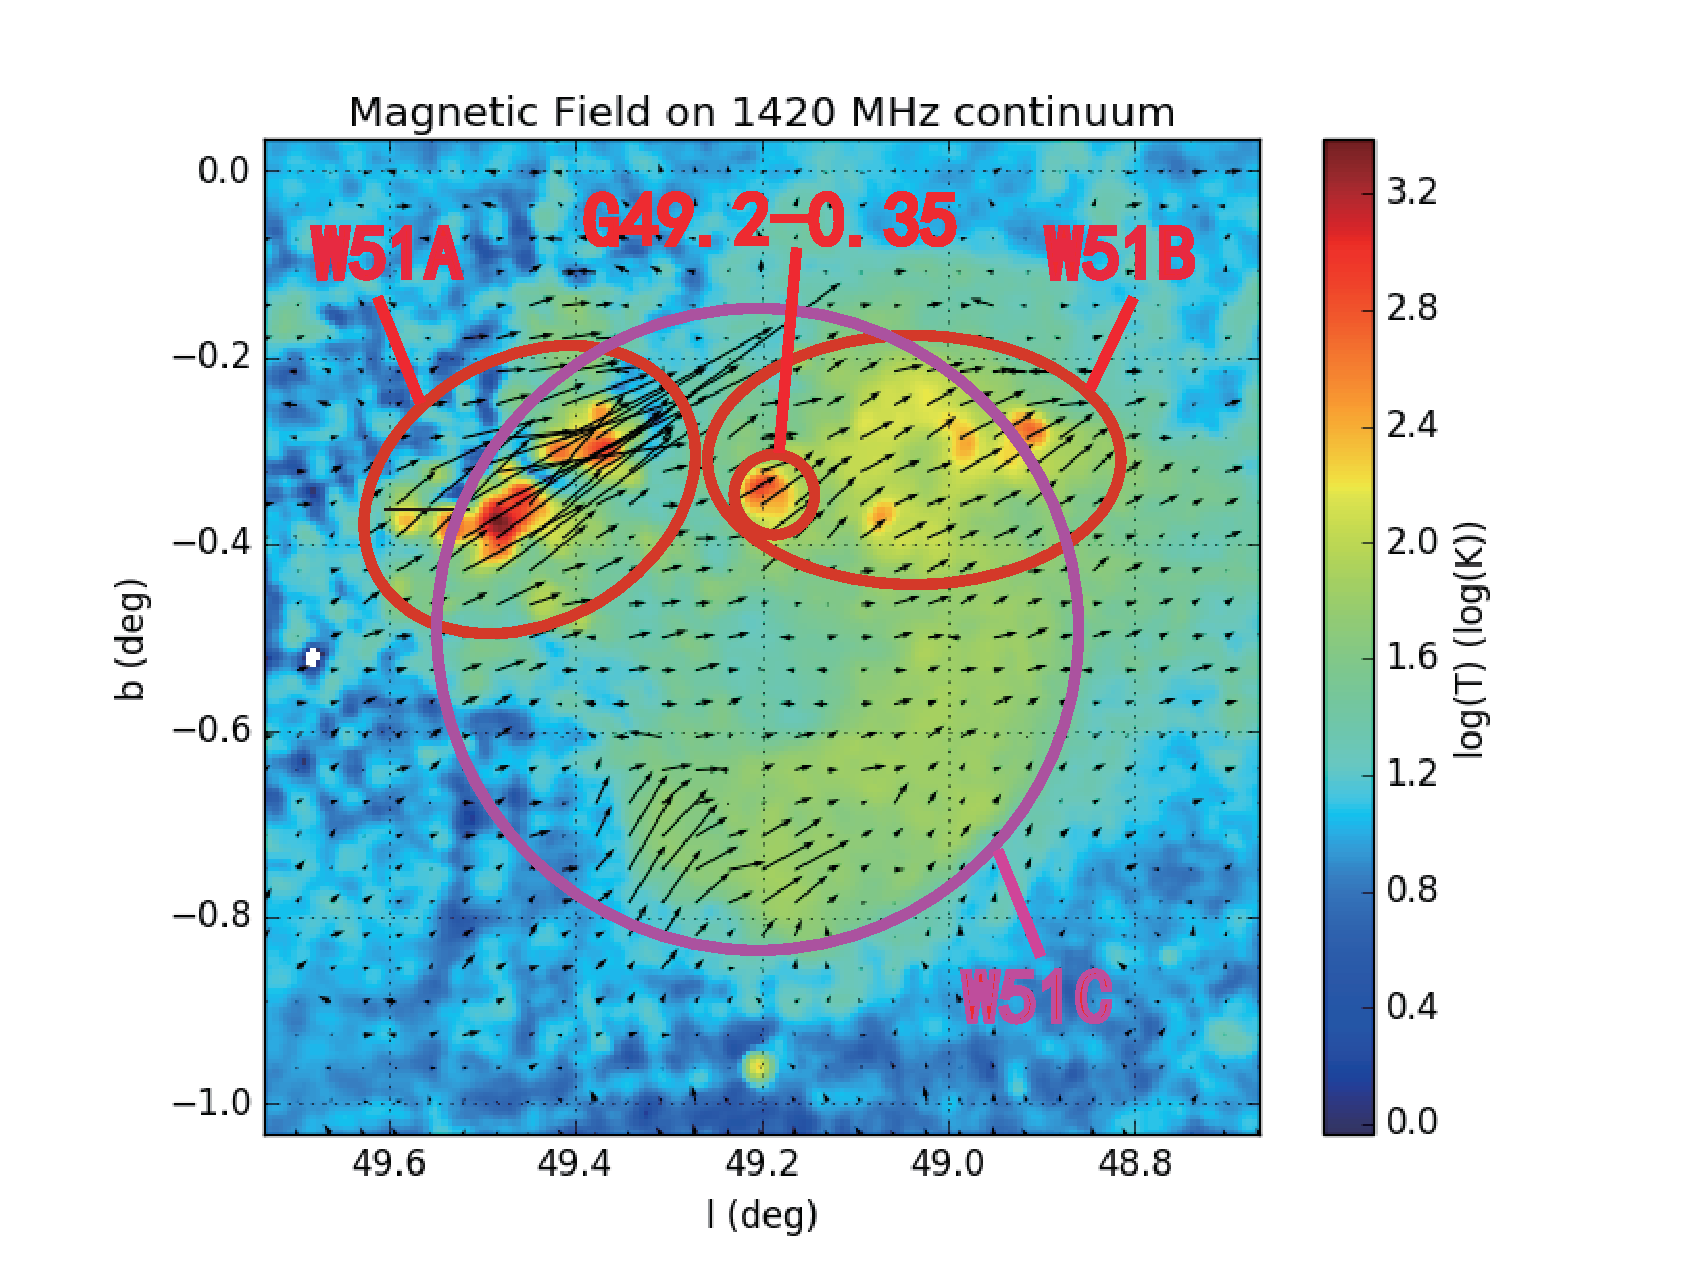
\includegraphics[width=0.495\textwidth]{mag0.eps}
   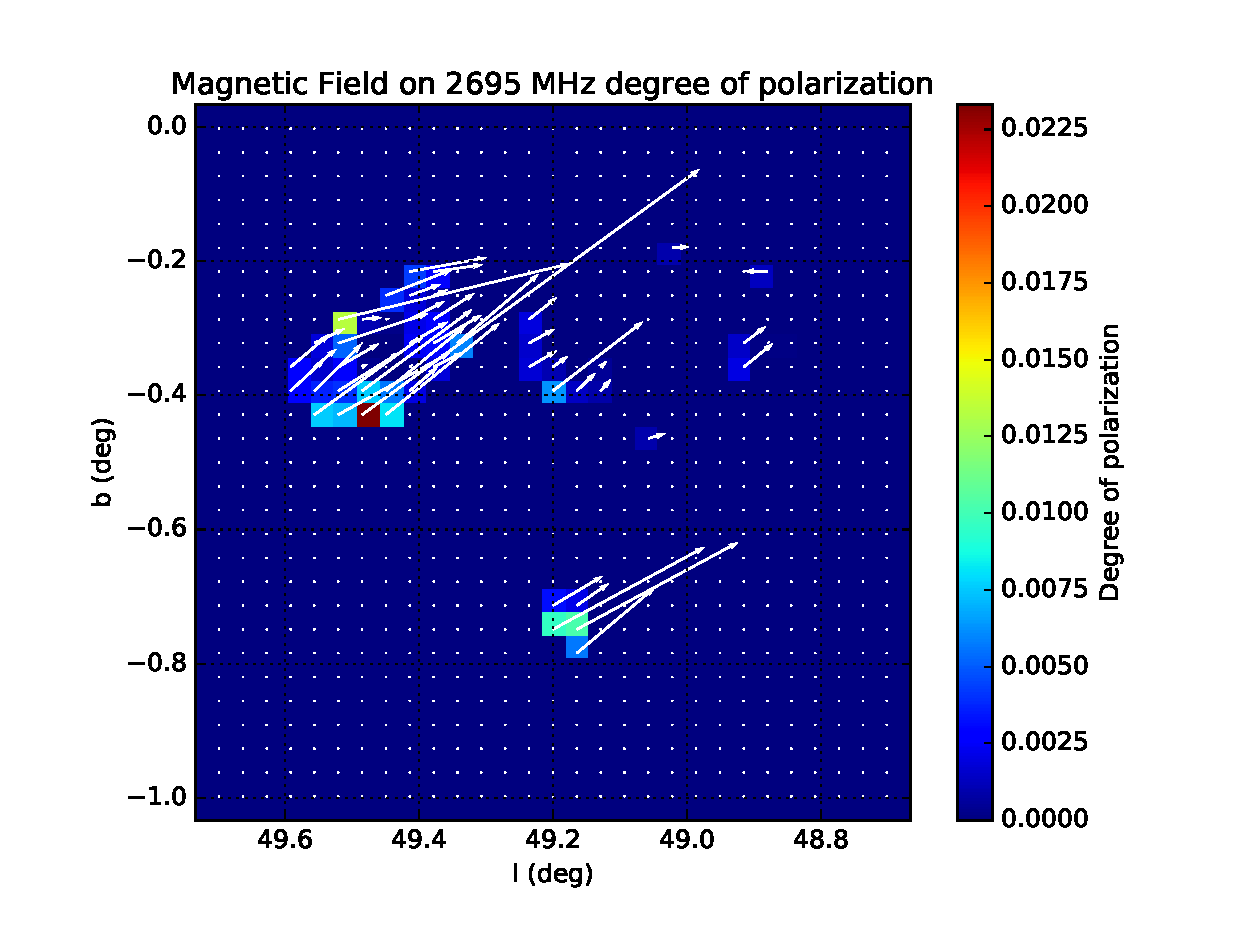
\includegraphics[width=0.495\textwidth]{modi_mag.eps}
   \caption{左侧图像中,彩色背景是1.4GHz的来自VGPS的连续谱图像,黑色的箭头代表磁场,箭头
   长度代表偏振强度(mK),最强处为1581mK,箭头方向代表磁场方向。
   右侧图像中彩色背景是在2695MHz处的偏振度,白色的箭头代表磁场,箭头
   长度代表偏振度,最强处为$2\%$,箭头方向代表磁场方向。
   }
\label{fig:mag}
\end{figure*}

\section{模拟模型}
\label{W51Cmod}
这里我们使用三维磁流体模拟,忽略了粘滞度、电阻、热传导等耗散效应,引力和辐射冷却也不予考虑,
而具体的参数大多来源于前人的观测。
\citet{Sasaki2014}使用6 kpc作为距离估计SNR W51C前身星的质量超过20 M$_\odot$。
这个距离是一个上限,所以真实的质量可能更小。
在这个模拟中,我们取20 M$_\odot$为前身星质量,这样其爆发时抛射物的质量就是11 M$_\odot$
\citep{Sukhbold2016}。
\citet{Koo1995}也使用6 kpc为距离估计其爆发能量为3.6 $\times$ 10$^{51}$ ergs s$^{-1}$,
这个完全超出了典型的爆发能量,1 $\sim$ 3 $\times$ 10$^{51}$ ergs s$^{-1}$ \citep{Poznanski2013}。
根据\citet{Poznanski2013}的工作,对于W51C,爆发能量大约为1.0 $\times$ 10$^{51}$ ergs s$^{-1}$
是比较合理的。
虽然 \citet{Poznanski2013}只是估计了通过估计一些SNRs的动能得出这样的经验关系,可是他用的
遗迹都非常年轻,或者更合理的说是刚爆发的超新星,所以其动能几乎等于其总爆发能量。
而在我们的模拟中也是如此认为,即使如今观测到的遗迹热能与动能相当,我们认为爆发时总能量
几乎全部来自动能,爆发时的动能就是如今热能与动能的总和。
在对W51C的流体模拟中,我们认为对结果起作用的主要是动能,热能导致的辐射耗散影响不大。
实际上,W51C是一个中等年龄的遗迹,因此他的爆发能量应该是现如今动能和热能之和。
\citet{Koo1995}根据X-ray观测先推出热能,然后根据Sedov模型估算总的爆发能量\citep{1959sdmm.book.....S}。
采用最近测量的4.3 kpc的距离\citep{Tian2013},我们采取了与\citet{Koo1995}相同的方法
得到了1.3 $\times$ 10$^{51}$ ergs s$^{-1}$的爆发能量,这是一个相对来说更合理的结果。
当然,SNRs的爆发能量其实变化很大,所以这并不能作为一个决定性的证据说明哪个距离就是正确的。
4.3 kpc在目前看来只是更可靠一点,所以我们在模拟中取其为W51C的距离。
我们选择$48.89^{\circ}<l<49.51^{\circ}$, $-0.81^{\circ}<b<-0.19^{\circ}$这一区域
作为模拟研究的目标。
这样对于这个大约角直径有37\am的遗迹,其真实直径是46 pc。
如果采用\citet{Koo1995}推导的平均激波速度490\kms,其年龄为18000年。

我们通过一个用于模拟SNR解析演化的Python计算器\citep{Leahy2017a}估计得到介质平均密度为
0.21 cm$^{-3}$。
为了模拟出介质的随机分布,我们采用了幂律的介质分布模型$N(\rho) = N_0 \rho^{-\alpha}$,
这里$N(\rho)$是像素数,表征了有某一个密度的格点的个数, $N_0$是一个常数,用来保证最终结果
满足平均密度估计,$\alpha$是一个幂律指数。
$\alpha$是正数,也就是说低密度的区域比高密度的区域更多更大。
举个粒子,在我们的模拟中,共有256 $\times$ 256 $\times$ 256个格点,那可能有一千万个点
密度低于0.21 cm$^{-3}$,而只有100个点密度高于21 cm$^{-3}$。
\citet{Parsons2012} 研究了SNR W51C周围的分子团块(包括致密团块),发现它们的质量分布
满足一个指数$\alpha$为2.4的幂律谱,这个结果暗含了真实的周围介质密度分布。
因为目前对这个区域没有原子氢密度分布的研究,所以我们取$\alpha=2.4$作为初始介质密度分布。
此外,为了模拟相互作用,我们在初始条件中加了一个密度为2 cm$^{-3}$直径为11 pc的分子云
(如图~\ref{fig:simulation}中间两幅图)。

\begin{figure*}
    \centering
    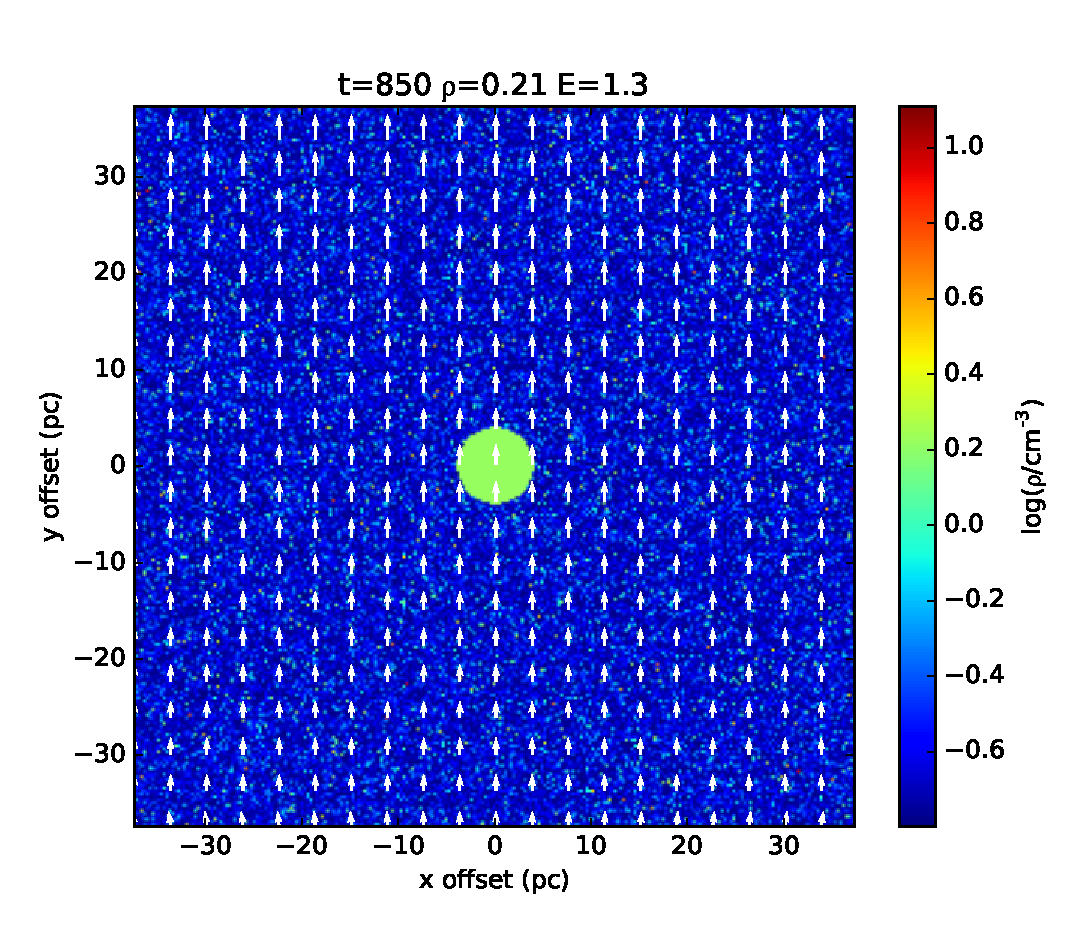
\includegraphics[width=0.323\textwidth]{rho850_density021_E13xy.eps}
    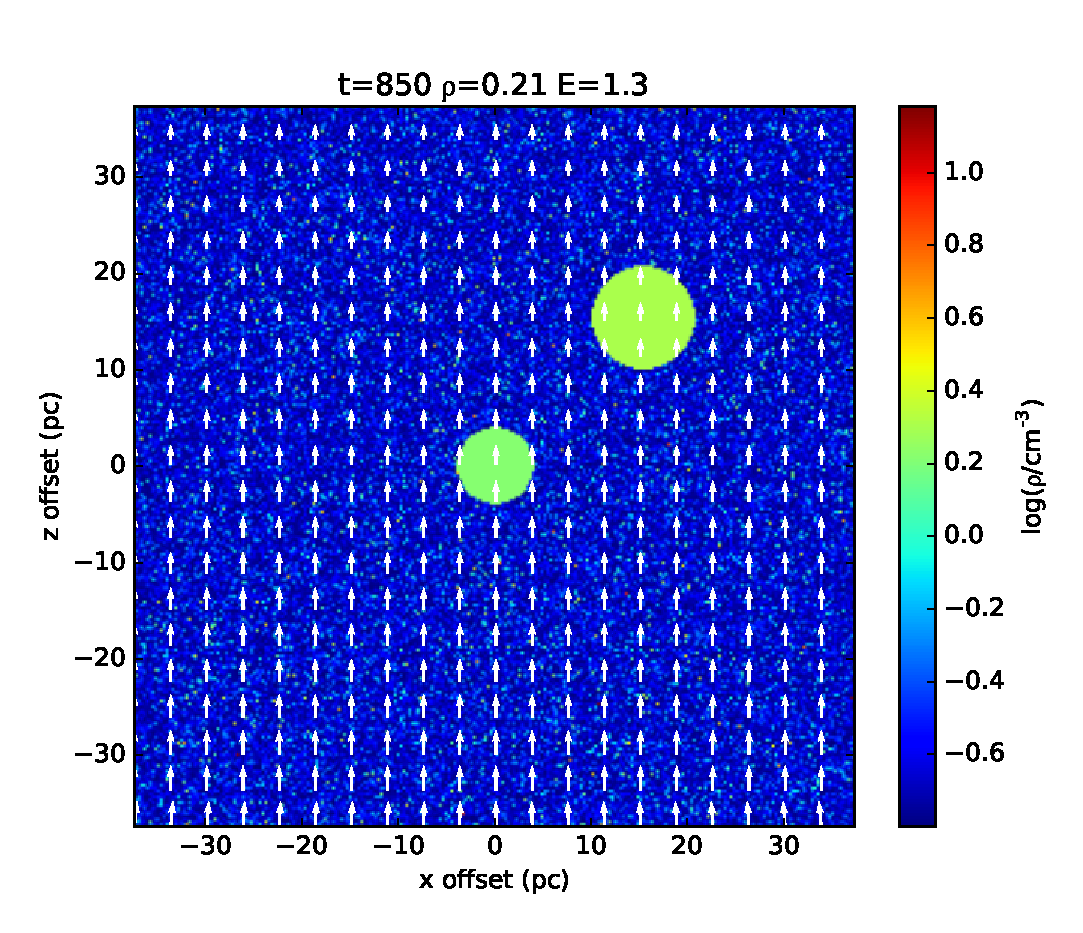
\includegraphics[width=0.323\textwidth]{rho850_density021_E13xz.eps}
    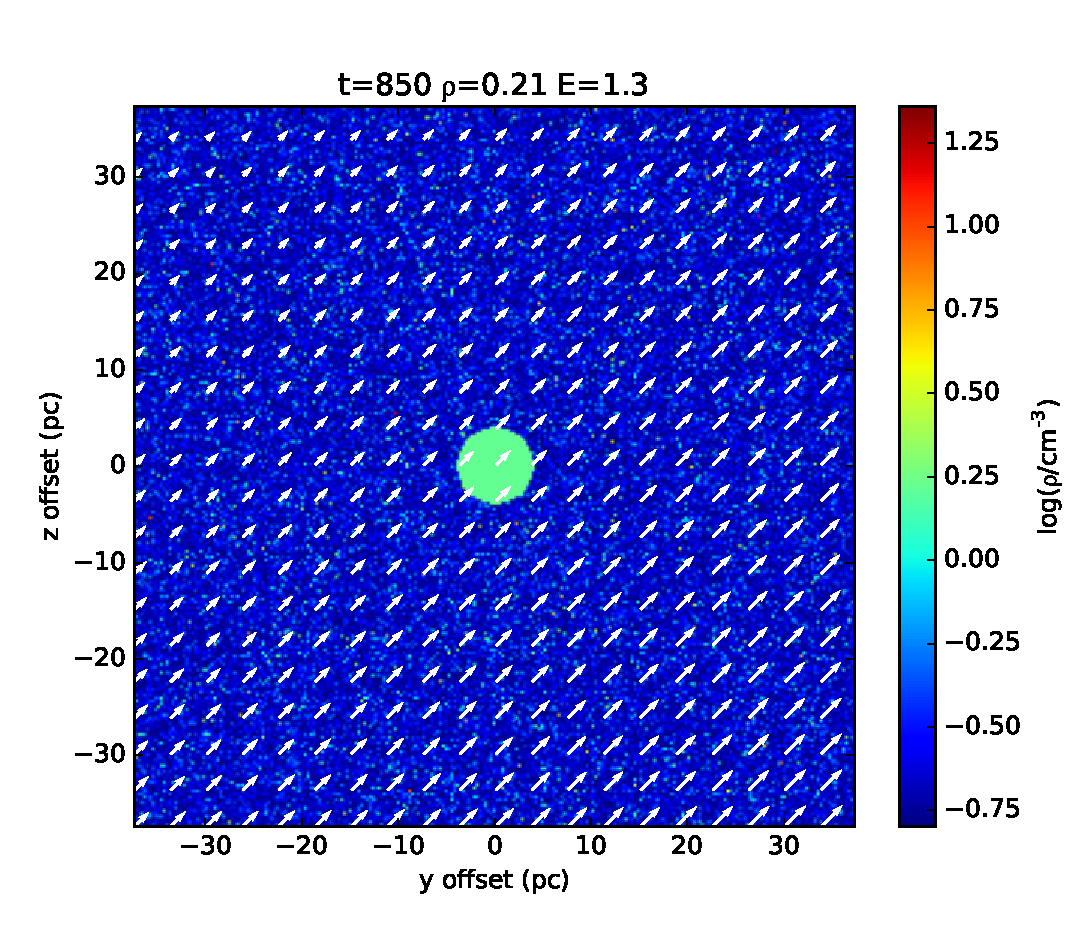
\includegraphics[width=0.323\textwidth]{rho850_density021_E13yz.eps}\newline
    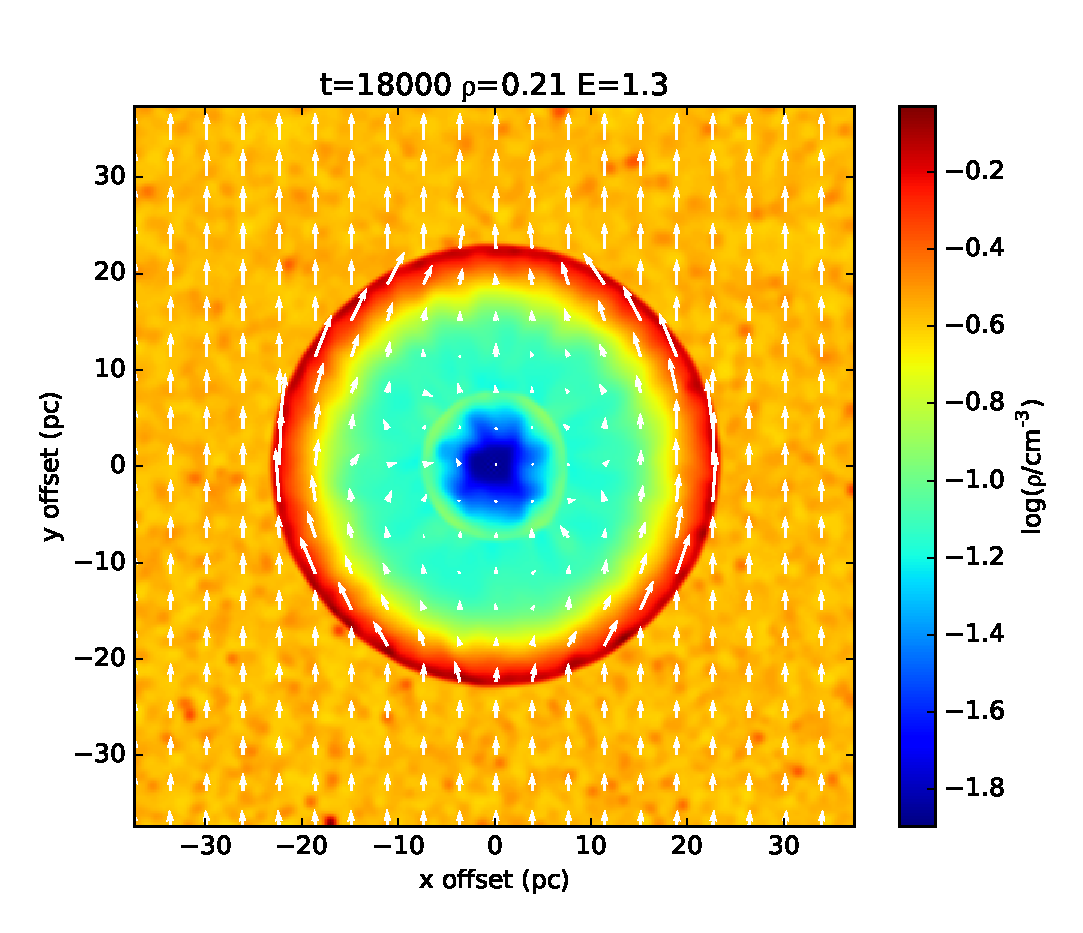
\includegraphics[width=0.323\textwidth]{rho18000_density021_E13xy.eps}
    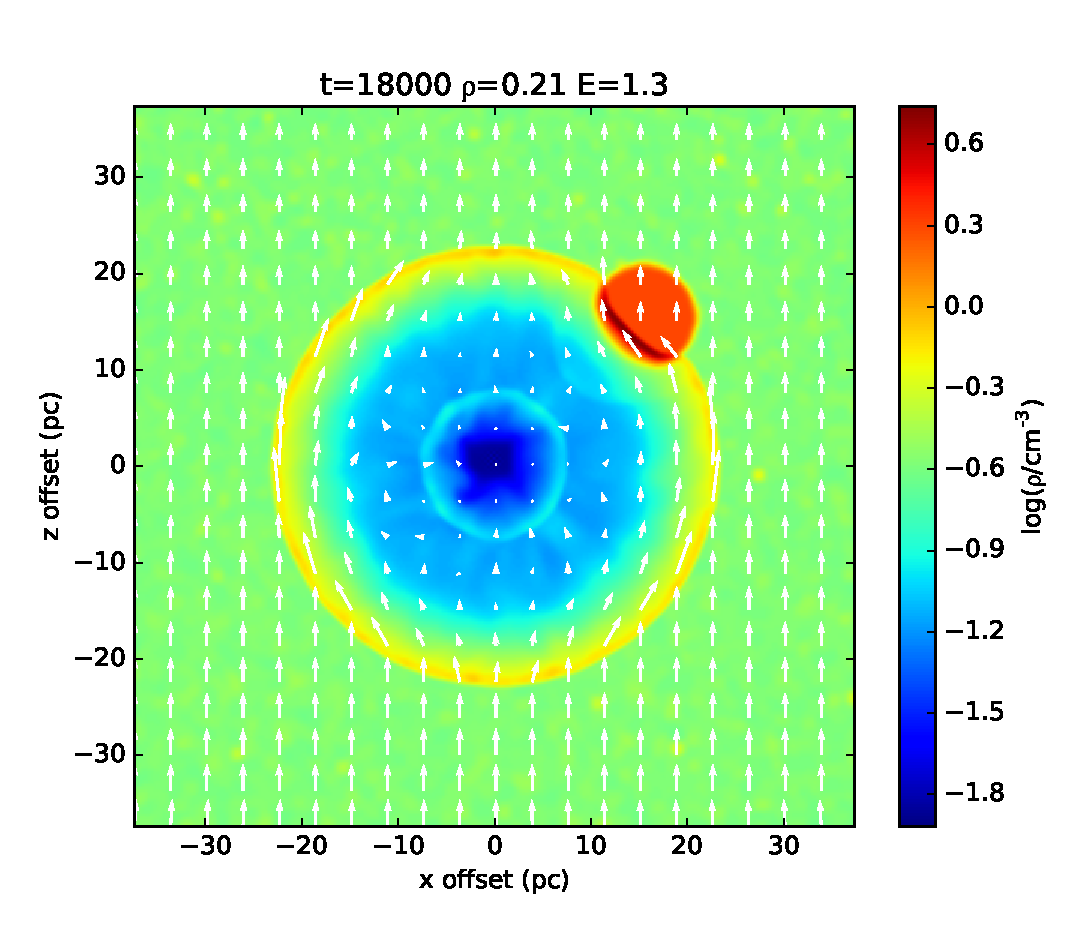
\includegraphics[width=0.323\textwidth]{rho18000_density021_E13xz.eps}
    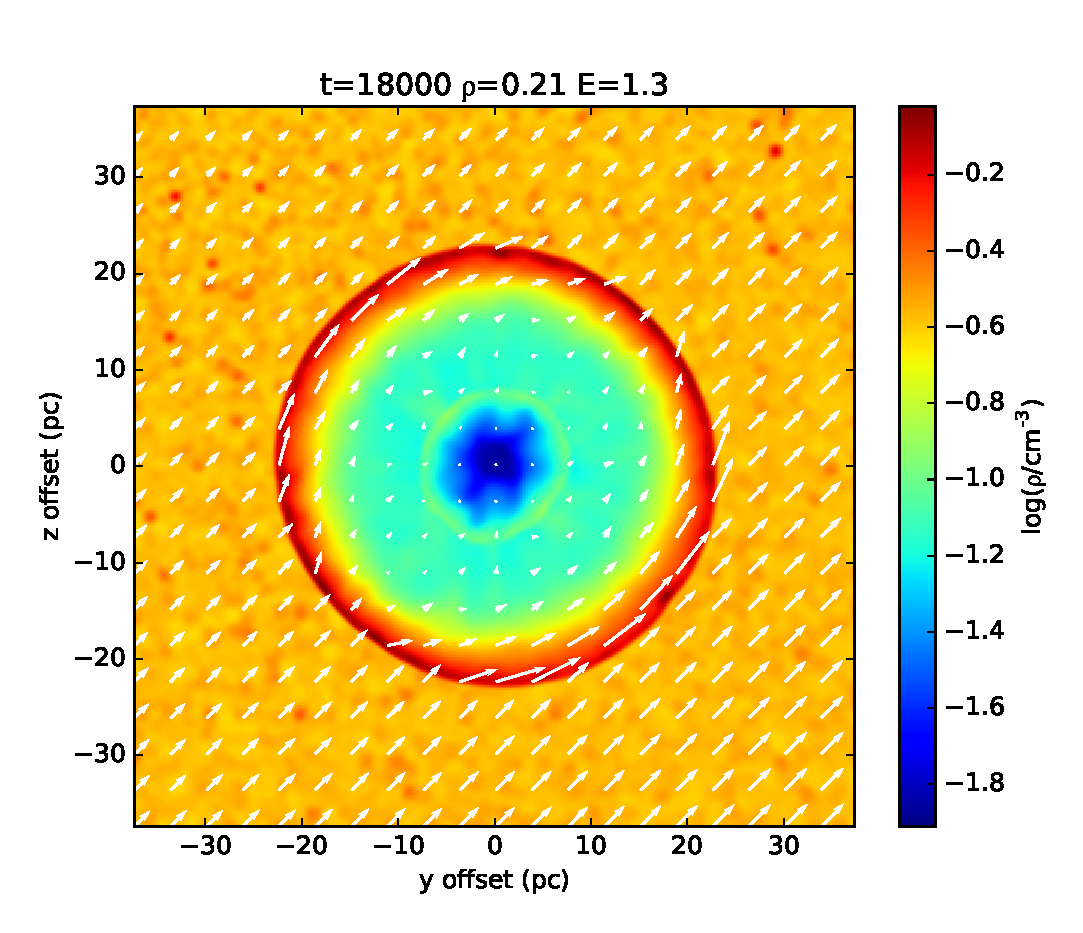
\includegraphics[width=0.323\textwidth]{rho18000_density021_E13yz.eps}
    \caption{模拟的密度-磁场图像。所有的图都是沿着一个三维立体图像沿着中心切片后得到的
    从不同方向看的结果。背景彩色图像是密度分布,白色箭头显示了磁场的方向和强度。上面三幅
    显示的是初始条件,下面三幅显示了经过18000年演化后的结果。上面三幅图中,中心磁场的强度
    是9$\mu G$。}
\label{fig:simulation}
\end{figure*}

因为W51C的壳层倾斜方向基本与银道面呈45$^{\circ}$夹角,所以我们在模拟中也设置了这样一个
角度。
我们在模拟中认为超新星爆发是球对称的,考虑到磁场,其遗迹的演化是柱对称的,所以为了产生一
个单边亮的壳层,我们需要设置不对称的初始介质分布,从而保证遗迹有一个边非常暗以至于其流量
低于射电望远镜观测灵敏度。
因为在这一区域我们并没有观测到明显的密度梯度分布,所以在这个模拟中,我们通过设置较大的磁
场梯度来保证一边流量大,一边流量小到观测不到。
而银河系介质中平均磁场强度为4 $\mu$G到14 $\mu$G \citep{Haverkorn2015},我们模拟的尺度
为$75 \times \sqrt{2}$ pc。
所以,我们假设模拟中心磁场强度为9 $\mu$G,而磁场梯度为0.1 $\mu$G pc$^{-1}$。
磁场梯度如果再大,最小磁场或者最大磁场就会超过比较合理的范围。

我们模拟了大小为$1^\circ \times 1^\circ$的区域,对于4.3 pc的距离实际尺度75 pc $\times$
75 pc。
对于这个区域,我们使用256 $\times$ 256 $\times$ 256的网格来进行三维模拟,也就是说,
其分辨率是0.3 pc pixel$^{-1}$ (0.24\am pixel$^{-1}$)。
因为模拟时网格为立方体,为了得到近似为球对称的爆发,我们需要设置较大的初始爆发半径。
同时,早期的自由膨胀相的遗迹演化可以通过解析解得到,而超过自由膨胀相的演化就不太适合了,
所以初始爆发半径又不能太大以至于演化到绝热膨胀相。
所以,对于W51C,我们选取初始爆发半径为4 pc,对于这个遗迹,它需要花费850年达到这个
半径,而他的绝热膨胀相起始于3200年\citep{Leahy2017a},所以它达到初始半径时仍处于自由
膨胀相。
在图~\ref{fig:simulation}中,上面三幅图展示了模拟中采用的初始条件。

为了与真实的观测图像相比较,我们假设其射电辐射全部来自于同步辐射,并使用简化公式
$i(\nu)=C\rho B_{\perp}^{\beta + 1}\nu^{-\beta}$ \citep{Orlando2007}得到相对射电
流量体密度,这里$\nu$是辐射频率,C是一个常数,$\rho$是密度,$B_{\perp}$是垂直于视线方
向的磁场,$\beta$是同步辐射谱指数。
通过沿视线方向积分,$\int i(\nu) \mathrm{d}l$,我们可以获得可以与实际观测相比较的相对
射电流量密度。
在我们的三维模拟中,X轴被定义为视线方向。
对于相互作用区域,我们认为大约10$\%$的介质对射电流量密度有贡献,也就是说
$i(\nu)=0.1C\rho B_{\perp}^{\beta + 1}\nu^{-\beta}$。
$\nu$取1.4GHz,$\rho$和$B_{\perp}$是模拟过程中的主要变量,$\beta$对于W51C取0.25
\citep{1970AuJPA..14..133S}。
然后我们可以获得一个相对射电流量密度的图像,而要获得绝对射电流量密度需要得知常数C,这个
对于每个遗迹都不一样,因为其中包含了激波加速效率等变量,这些量对于每个遗迹都不一样,
要获得C需要将观测与模拟相对比得到。
但是相对射电流量已经能够告诉我们很多信息了。
用于比较的VGPS射电连续谱的分辨率是1\am,而模拟结果分辨率高很多,如果要将其与模拟结果比较
的话,需要将模拟结果分辨率平滑到与观测相近。
分辨率其实指的是观测源的半高全宽(the full width at half maximum, FWHM),对于用于平滑的
高斯方程:

\begin{equation}
  \begin{aligned}
    G(x)=\dfrac{1}{\sigma \sqrt{2\pi}}e^{-\dfrac{1}{2}(\dfrac{x-\mu}{\sigma})^2},
  \end{aligned}
\end{equation}

其FWHM定义为$2\sqrt{2ln2} \sigma$。
对于VGPS,其$\sigma$为0.42\am,我们模拟的分辨率是0.24\am pixel$^{-1}$,所以用于平滑
的$\sigma$为0.42\am/0.24\am pixel$^{-1}$=1.75 pixel,作为简化,我们取$\sigma$=2
pixel。

这个工作中我们模拟了SNR W51C演化18000年的结果,主要使用的参数都列在表~\ref{table:parameters}
中,其中没有参考文献的参数都来自于我们的估计。
当然,我们在模拟中也尝试过不同的参数,比如设置爆发能量为2.0和3.0 $\times$ 10$^{51}$ erg,
设置平均密度为0.13 cm$^{-3}$和0.3 cm$^{-3}$,设置谱指数为1.0和3.0。

\begin{table*}
  \caption{用于W51C模拟的参数}
  \label{table:parameters}
  \centering
  \begin{tabular}{l l l}
      \hline\hline
      参数                         & 值           & 参考文献               \\
      \hline
      抛射质量                      & 11 M$_{\odot}$ & 1, 2\\
      初始爆发动能                  & 1.3$\times$ 10$^{51}$ ergs & 3, 4\\
      模拟初始半径                  & 4 pc            &\\
      模拟起始时间                  & 850 years       & 5\\
      \hline
      平均密度                      & 0.21\ cm$^{-3}$ & 4, 5\\
      密度分布指数 ($\alpha$)       & 2.4             & 6\\
      磁场梯度                      & 0.1 $\mu$G pc$^{-1}$    &\\
      中心磁场强度                  & 9 $\mu$G        &\\
      平均原子质量                  & 1.3             &\\
      绝热系数                      & 5/3             &\\
      温度                         & 100 K           &\\
      \hline
      同步辐射谱指数 ($\beta$)       & 0.25            & 7\\
      距离                          & 4.3 kpc         & 8\\
      \hline
  \end{tabular}\\
  \tablerefs{(1)\citealt{Sasaki2014}; (2)\citealt{Sukhbold2016}; (3)\citealt{Poznanski2013}; (4)\citealt{Koo1995};
  (5)\citealt{Leahy2017a}; (6)\citealt{Parsons2012}; (7)\citealt{1970AuJPA..14..133S}; (8)\citealt{Tian2013}}
\end{table*}




\section{模拟结果}

\begin{figure*}
    \centering
    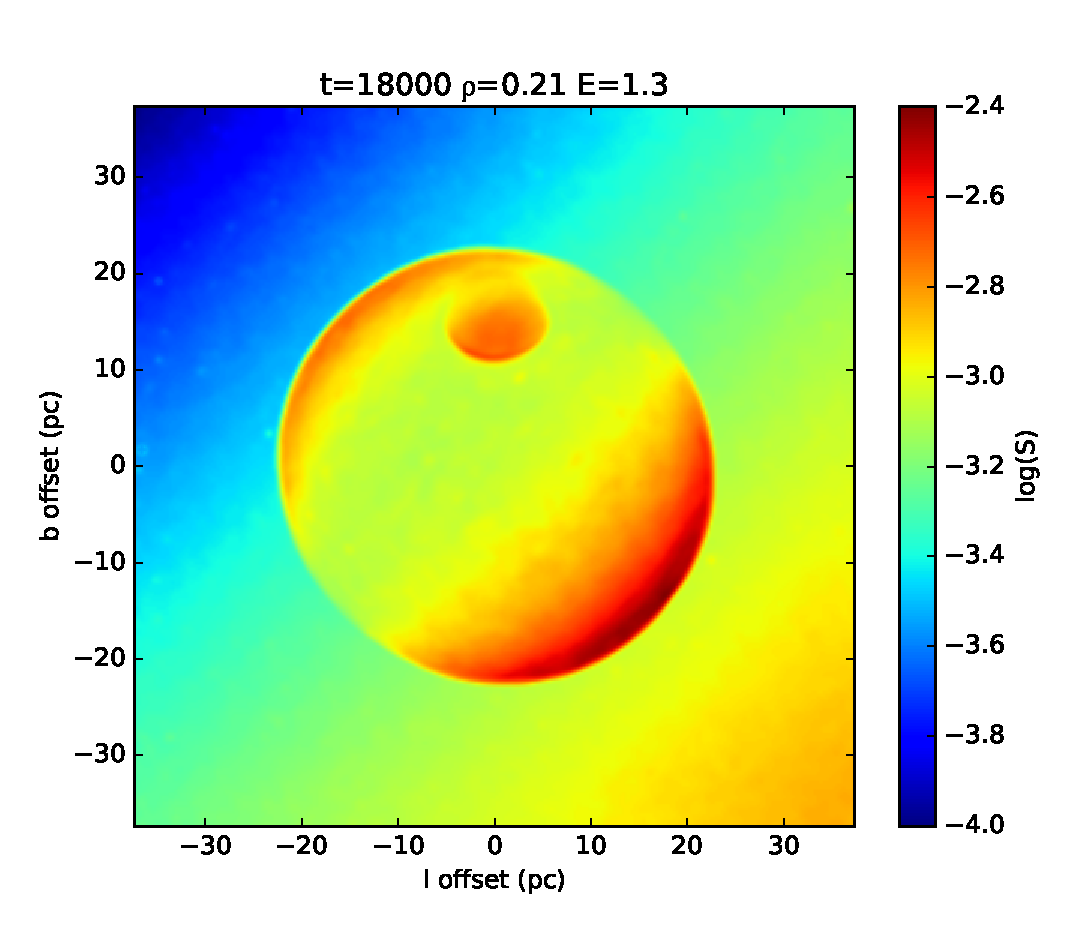
\includegraphics[width=0.472\textwidth]{t18000_density021_E13_s0.eps}
    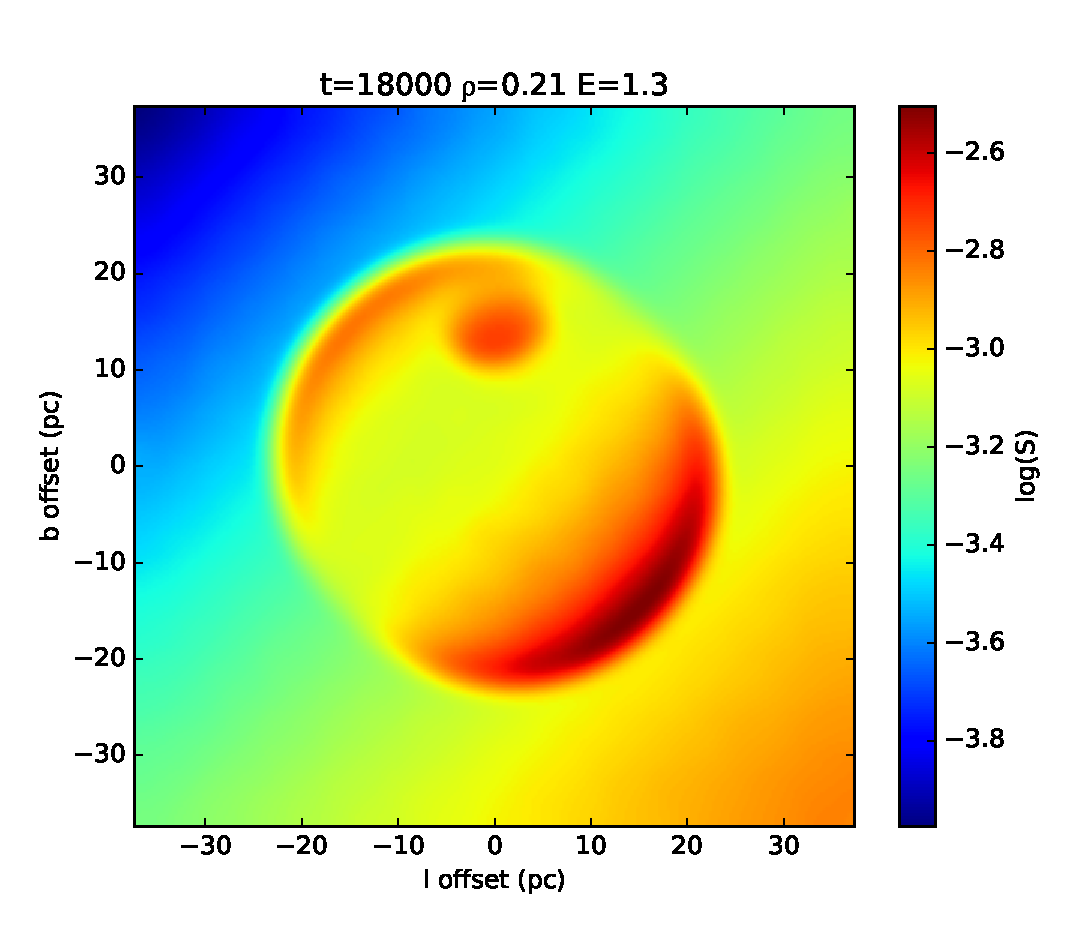
\includegraphics[width=0.472\textwidth]{t18000_density021_E13_s4.eps}
    \caption{SNR W51C演化18000年后的相对射电流量密度。右侧图像是$\sigma$=2的高斯平滑结果。
    这里设定距离为4.3 kpc,所以1 pc对应着0.8\am。}
\label{fig:flux}
\end{figure*}

主要的模拟结果在图~\ref{fig:simulation}中,我们能看到两侧激波区和相互作用区域有明显的
磁场放大。
在y-z平面中,左上角和右下角壳层的磁场强度大于他们的周围区域,右下角的磁场大于左上角的。
遗迹内部的密度和磁场强度都变得很低,外部壳层很致密,并有很强的磁场。
此外,遗迹内部有一层磁场密度比外壳层低,但是明显比周围要高一些的薄薄的壳层。

\begin{figure*}
    \centering
    \includegraphics[width=0.472\textwidth]{change.eps}
    \caption{这是图~\ref{fig:flux}的右图中左上到右下的流量切线图。 }
\label{fig:change}
\end{figure*}

图~\ref{fig:flux}是从密度图转化而来的相对射电流量密度图,用的谱指数是2.4。
我们也测试过谱指数为1.0和3.0的模拟。
谱指数为1.0时,射电图像呈现更过随机成分,但是别的特征与使用2.4时相似。
谱指数为3.0时,射电图像与使用2.4时并无太大差别。
因此,我们只在这里展示使用谱指数为2.4的图像。
左侧是直接转化的图像,右侧是使用$\sigma$=2高斯平滑后的图像。
可见左上角的壳层弱了很多,但明显还是有一定辐射。
图~\ref{fig:change}是图~\ref{fig:flux}中右图沿着左上到右下的流量密度变化,这显示出
左上角辐射流量密度大约是右下角的一半,而其实我们期待它应该更少。
遗迹区域中心流量是最低的,此外相互作用区也有明显的辐射。
图~\ref{fig:moreflux}展示了不同参数下的模拟结果。

\begin{figure*}
    \centering
    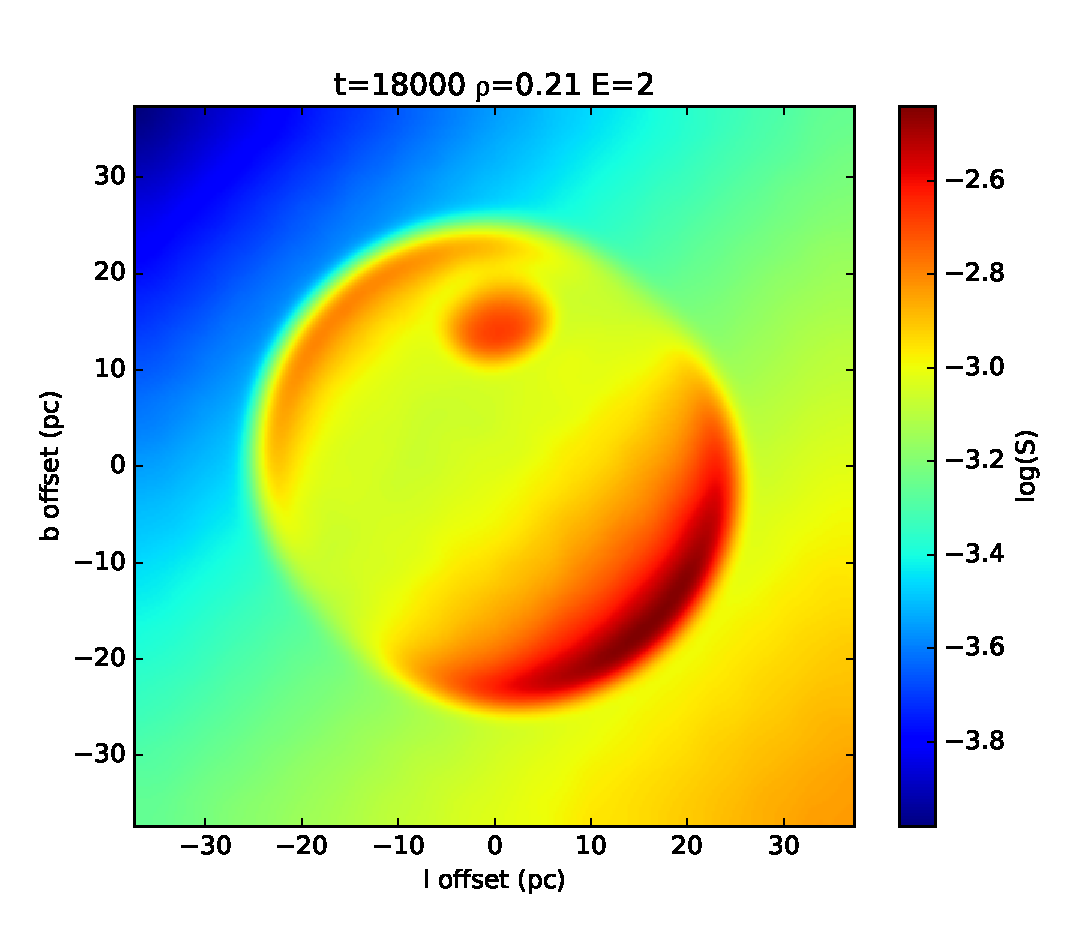
\includegraphics[width=0.472\textwidth]{t18000_density021_E2.eps}
    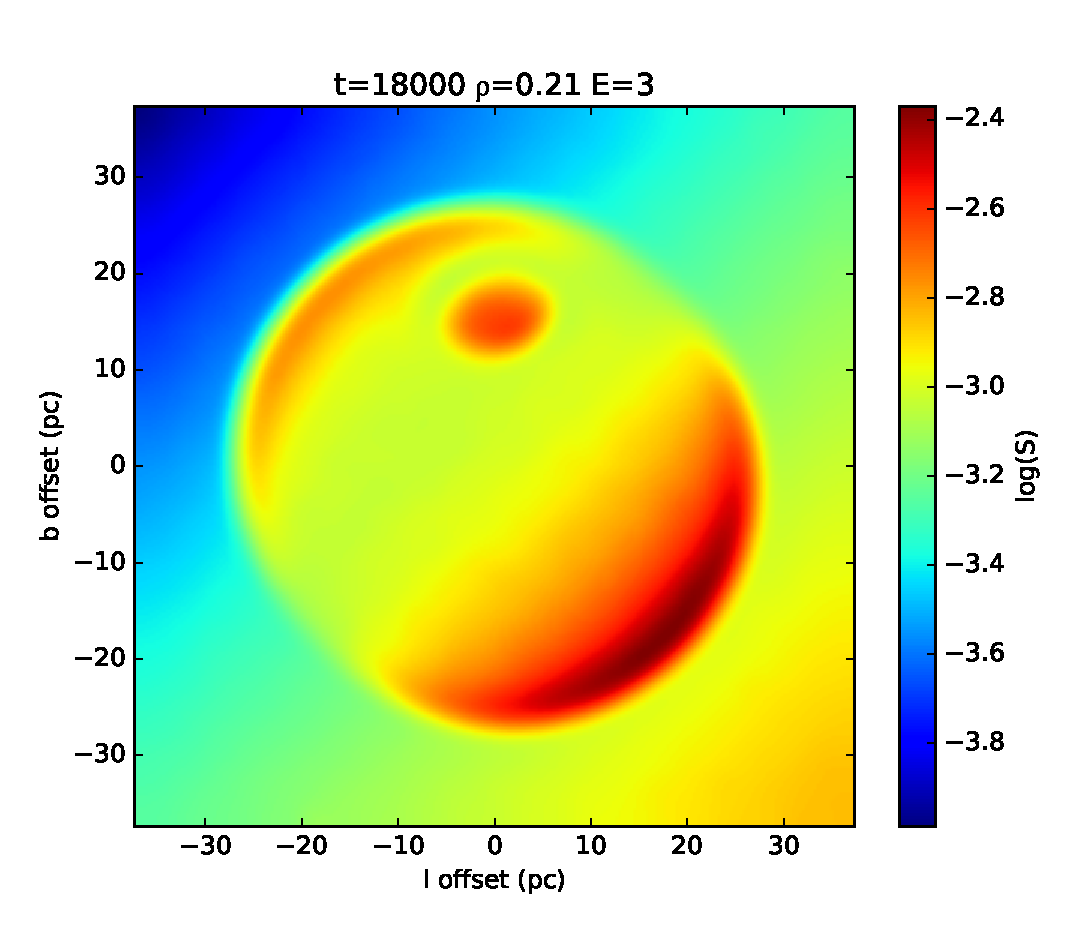
\includegraphics[width=0.472\textwidth]{t18000_density021_E3.eps}\newline
    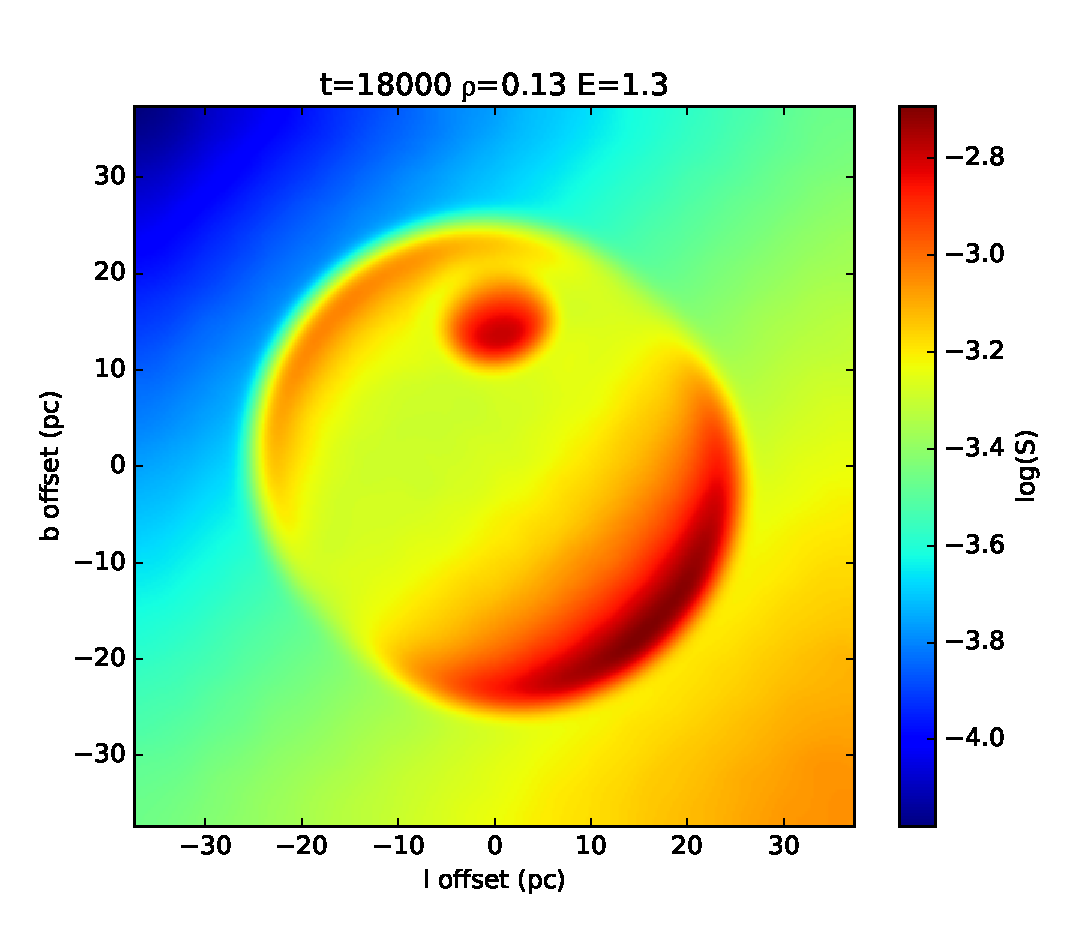
\includegraphics[width=0.472\textwidth]{t18000_density013_E13.eps}
    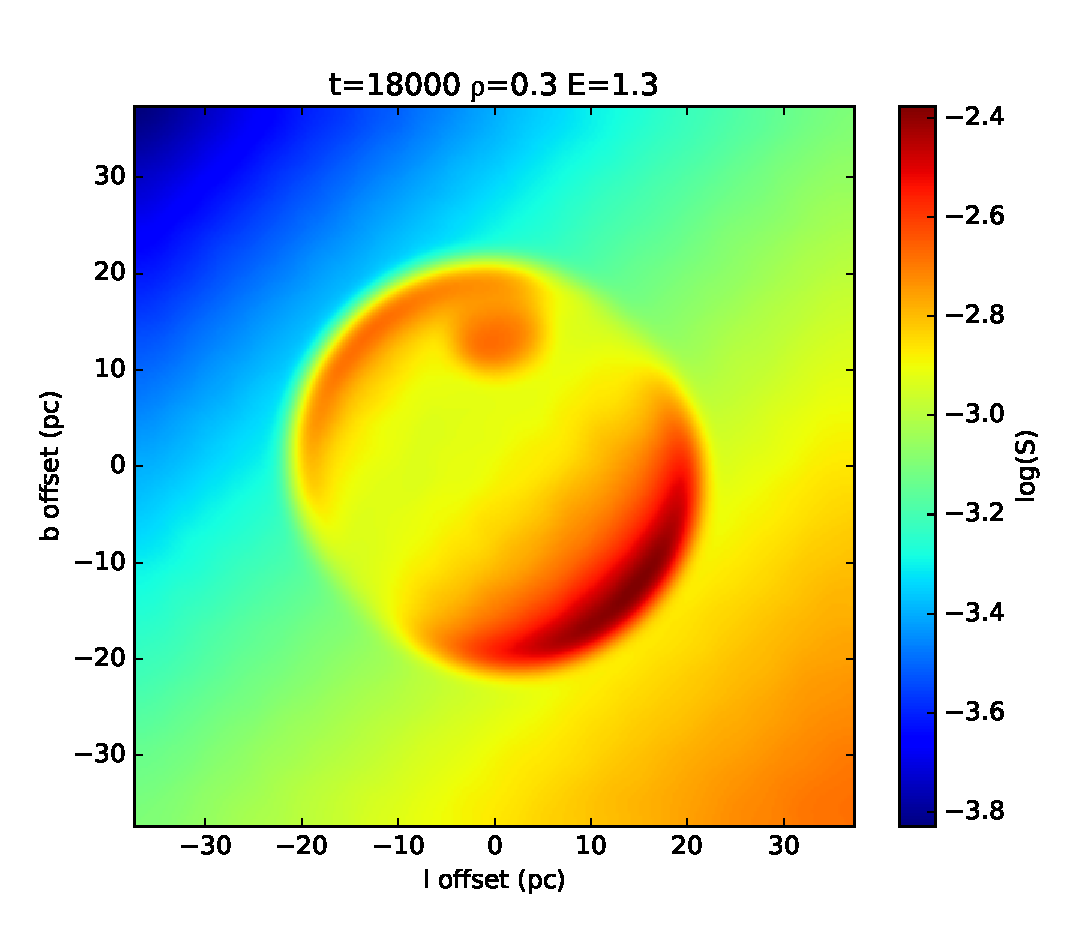
\includegraphics[width=0.472\textwidth]{t18000_density03_E13.eps}
    \caption{这是$\sigma$=2时不同参数下的相对射电流量密度图。 顶部两幅图为将初始爆发动能改为
    2.0和3.0 $\times$ 10$^{51}$ ergs的结果, 下面两幅图为将平均介质密度改为
    0.13 cm$^{-3}$和0.3 cm$^{-3}$的结果。}
\label{fig:moreflux}
\end{figure*}

图~\ref{fig:mag}是W51C实际观测到的磁场结构。
我们能看到其中有四个区域有很强的偏振:东北(NE)、中部(M)、西北(NW)、南部(S)。
这四个区域的磁场方向相近,只有东北的方向有点小混乱,同时东北区的偏振是最强的。
去除仪器偏振之后,西北区域的偏振基本不见了,而其它三个区域的偏振仍然存在,这三个区域东北
、中部、南部分别对应实际的三个源W51A、G49.2-0.35、W51C。
此外,去除仪器偏振后,东北区的偏振变得规则了,这可能意味着我们已经去除了足够的仪器偏振。

\begin{figure*}
   \centering
   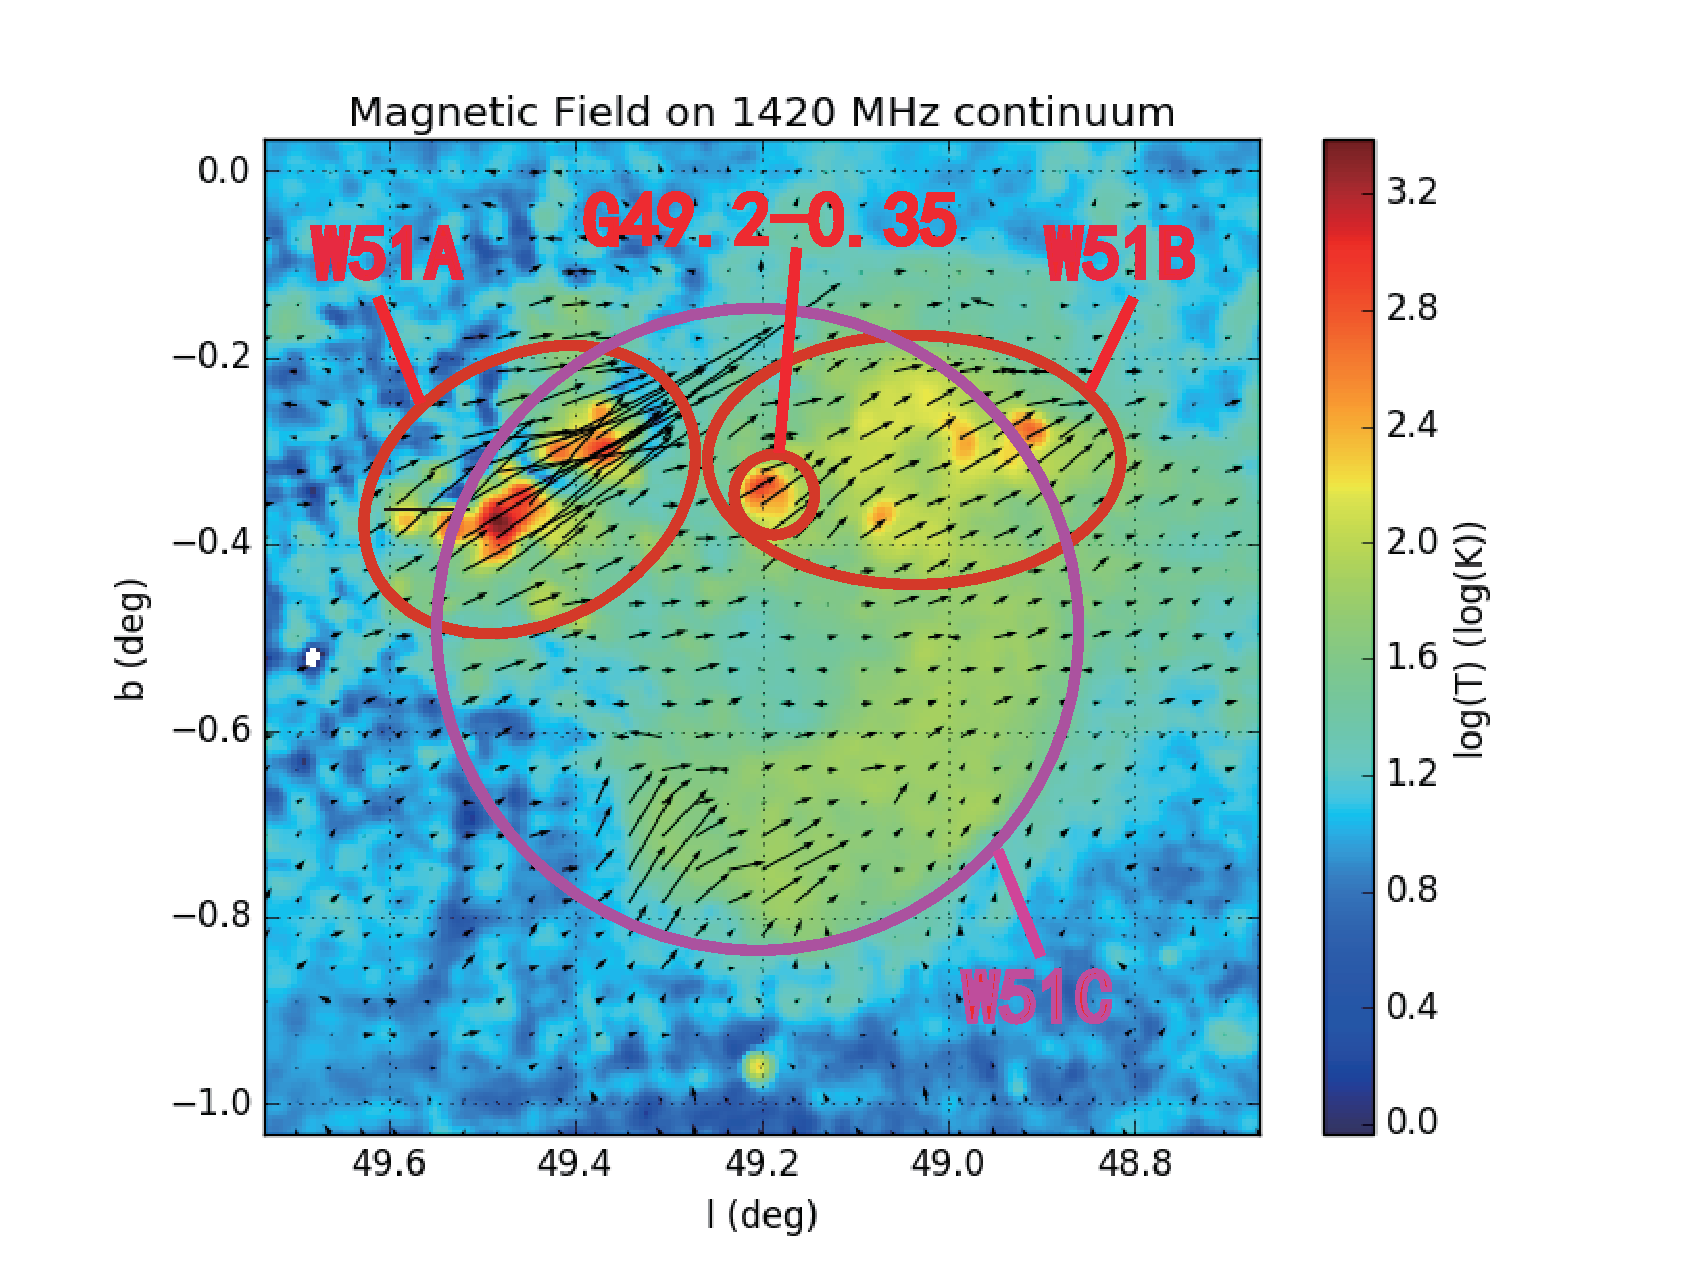
\includegraphics[width=0.472\textwidth]{mag0.eps}
   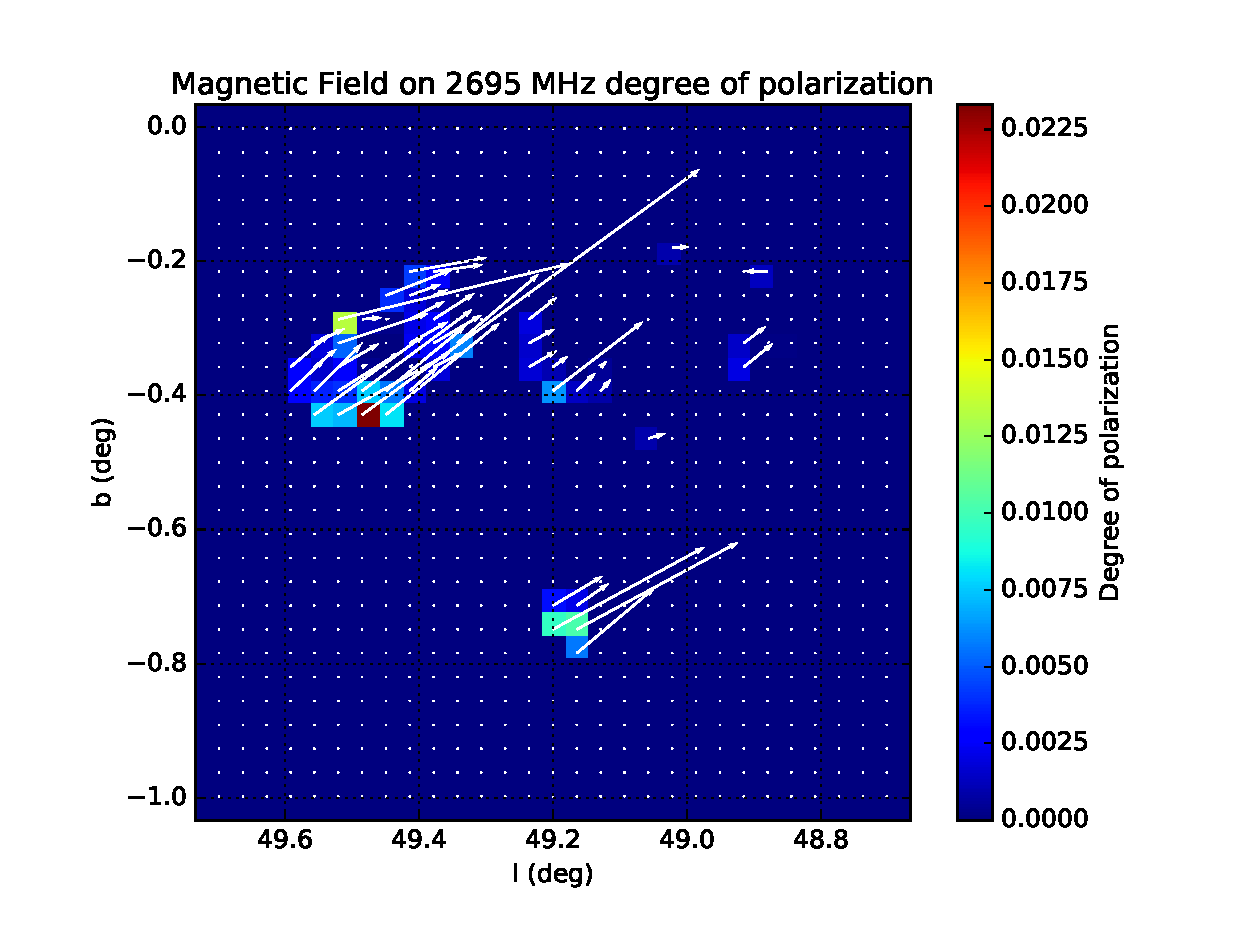
\includegraphics[width=0.472\textwidth]{modi_mag.eps}
   \caption{左图中彩色背景是来自VPGS的1.4 GHz连续谱图像。黑色的箭头代表没有扣仪器偏振的
   在2695 MHz的磁场方向,箭头长度代表偏振强度(mK),其中最大的强度是1581 mK。
   下图中,彩色背景是扣除仪器偏振后的2695 MHz的偏振度,白色箭头代表磁场方向,箭头长度代表
   偏振度,其中最大的偏振度是$2\%$。}
\label{fig:mag}
\end{figure*}

之前,对这个区域已经有高分辨率的1720 MHz的观测\citep{2005ASPC..340..334B},但是还没
有与之对应的高分辨率的1665/1612 MHz观测。
这几个频率是羟基分子(OH)在射电波段的主要跃迁频率,对于我们研究超新星遗迹与分子云相互作用
有重要研究价值。
而THOR数据极高的分辨率提供给我们绝佳的机会来揭示1720 MHz辐射与 1720/1665/1612 MHz吸收的
空间位置关系。
图~\ref{fig:OH}是这个区域羟基OH的谱线图,彩色背景是THOR 1.4 GHz的连续谱图像,白色的
谱线为每个黑色方格中的平均结果。
其中,1720 MHz OH 脉泽非常强,而且明显距W51B中的小电离氢区G49.2-0.35一定距离。
当然,这里我们要说明,我们模拟中的相互作用区域的射电辐射与这个小电离氢区的射电辐射不是一
件事,实际观测到的射电辐射可能是电离氢区与相互作用区域在视线方向重合后相互叠加的效果。
事实上,我们并没有直接探测到相互作用区域的射电辐射,但是1720 MHz OH脉泽和微弱但确实存在
的射电偏振辐射让我们认为它确实存在。
G49.2-0.35中射电亮的区域也呈现出明显的1720/1665/1612 MHz OH 吸收线,然而射电暗的区域却
呈现出较宽的发射线而且1665 MHz OH 辐射非常强。
同时,有一些发射和吸收特征明显远离这个小电离氢区,所以应该是与周围前景或背景有关,这让我
们猜测G49.2-0.35的前景或背景会一定程度上影响我们看到的G49.2-0.35区域的谱线。
不过,虽然谱线来源或许不同,但是其特征速度都相似,因此


\section{羟基谱线分析}
\section{讨论}
